\documentclass[letterpaper]{article}

% ==================================================
% PACKAGE
% ==================================================

\usepackage{graphicx}
\usepackage{fontspec}
\usepackage{geometry}
\usepackage{titlesec}
\usepackage{titletoc}
\usepackage{indentfirst}
\usepackage{caption}
\usepackage{fancyhdr}
\usepackage[
    style=apa,
    backend=biber
    ]{biblatex}
\usepackage{float}

% ==================================================
% FONT
% ==================================================

\setmainfont{Times New Roman}

% ==================================================
% PAGE
% ==================================================

\geometry{
    letterpaper,
    left=2.54cm,
    right=2.54cm,
    top=2.54cm,
    bottom=2.54cm
}

% ==================================================
% NUMBERING
% ==================================================

% Section:
% A.
% B.
% C.
\renewcommand{\thesection}{\Alph{section}.}

% Subsection:
% 1.
% 2.
% 3.
\renewcommand{\thesubsection}{\arabic{subsection}.}

% Subsubsection:
% 1.1.
% 1.2.
% 2.1.
\renewcommand{\thesubsubsection}
    {\arabic{subsection}.\arabic{subsubsection}}

% ==================================================
% JUDUL SECTION
% ==================================================

% --------------------------------------------------
% SECTION
% --------------------------------------------------

\titlecontents{section}
    [0cm]
    {}
    {\contentslabel{0.6cm}}
    {}
    {\titlerule*[0.7pc]{.}\contentspage}

\titleformat{\section}
    {\normalfont}
    {\makebox[0.5cm][l]{\thesection}}
    {0pt}
    {}

\titlespacing*{\section}
    {0pt}
    {2.0ex}
    {1.0ex}


% --------------------------------------------------
% SUBSECTION
% --------------------------------------------------

\titlecontents{subsection}
    [0.6cm]
    {}
    {\contentslabel{0.6cm}}
    {}
    {\titlerule*[0.7pc]{.}\contentspage}

\titleformat{\subsection}
    {\normalfont}
    {\makebox[0.5cm][l]{\thesubsection}}
    {0pt}
    {}

\titlespacing*{\subsection}
    {0.5cm}
    {1.5ex}
    {0.75ex}


% --------------------------------------------------
% SUBSUBSECTION
% --------------------------------------------------

\titlecontents{subsubsection}
[1.5cm]
{}
{\contentslabel{0.9cm}}
    {}
    {\titlerule*[0.7pc]{.}\contentspage}

\titleformat{\subsubsection}
    {\normalfont}
    {\makebox[0.75cm][l]{\thesubsubsection}}
    {0pt}
    {}

\titlespacing*{\subsubsection}
    {1cm}
    {1.5ex}
    {0.75ex}
    

% --------------------------------------------------
% CAPTION GAMBAR ATAU FOTO
% --------------------------------------------------

\DeclareCaptionFont{mycaptionfont}{%
    \itshape
    \fontsize{11pt}{13pt}\selectfont
}

\captionsetup[figure]{
    name=Gambar,
    labelsep=space,
    font=mycaptionfont
}

% Nomor gambar mengikuti:
% section.subsection.subsubsection
\renewcommand{\thefigure}{%
    \thesubsubsection\arabic{figure}%
}

\counterwithin{figure}{subsubsection}

% --------------------------------------------------
% FORMAT DAFTAR GAMBAR
% --------------------------------------------------

\renewcommand{\numberline}[1]{Gambar #1\hspace{0.25cm}}


% ==================================================
% PARAGRAF
% ==================================================

% Indentasi paragraf
\setlength{\parindent}{0cm}

% Jarak antarparagraf
\setlength{\parskip}{0pt}

% Tambahan ruang elastis agar baris tetap rapi
% pada paragraf dengan indentasi kiri yang dalam
\setlength{\emergencystretch}{3em}

% ==================================================
% DAFTAR ISI
% ==================================================

% Menghilangkan tulisan "Contents"
\renewcommand{\contentsname}{}

% ==================================================
% NOMOR HALAMAN
% ==================================================

\pagestyle{fancy}

\fancyhf{}

% Nomor halaman di tengah footer
\fancyfoot[C]{\thepage}

% Hilangkan garis header/footer
\renewcommand{\headrulewidth}{0pt}
\renewcommand{\footrulewidth}{0pt}

% ==================================================
% FORMAT DAFTAR PUSTAKA
% ==================================================

\DeclareLanguageMapping{english}{english-apa}

\addbibresource{references.bib}

% ==================================================
% Kustomisasi Biblatex APA 7th agar Case-Sensitive & Dinamis
% ==================================================

% 1. Mencegah biblatex mengubah judul artikel menjadi sentence case
\DeclareFieldFormat{title}{#1}
\DeclareFieldFormat[article]{title}{#1}
\DeclareFieldFormat[online]{title}{#1}

% 2. Memastikan organisasi/situs web, bulan, dan tahun tampil dengan benar
% (Biasanya otomatis jika field organization/publisher dan month/year terisi dengan benar di .bib)

% --------------------------------------------------
% HILANGKAN TANGGAL AKSES
% --------------------------------------------------

\AtEveryBibitem{%
    \clearfield{urldate}%
}

% --------------------------------------------------
% ELEMEN YANG DIMULAI PADA BARIS BARU
% --------------------------------------------------

% URL → selalu baris baru
\DeclareFieldFormat{url}{%
    \newline
    \url{#1}%
}

% Publisher → selalu baris baru
\DeclareListFormat{publisher}{%
    \newline
    #1%
}

% --------------------------------------------------
% SPACING
% --------------------------------------------------

\setlength{\bibitemsep}{0.25cm}
\setlength{\bibparsep}{0pt}

% --------------------------------------------------
% INDENTASI
% --------------------------------------------------

\defbibenvironment{bibliography}
{
    \list
        {}
        {
            \setlength{\leftmargin}{1.5cm}
            \setlength{\itemindent}{-1cm}
            \setlength{\labelsep}{0pt}
            \setlength{\rightmargin}{0pt}
            \setlength{\listparindent}{0pt}
            \setlength{\parsep}{0pt}
            \setlength{\itemsep}{0.25cm}
        }
}
{\endlist}
{\item}

% ==================================================
% DOKUMEN
% ==================================================

\begin{document}

% ==================================================
% HALAMAN JUDUL
% ==================================================

\begin{titlepage}

    \pagenumbering{Roman}
    \setcounter{page}{1}

    \begin{center}

        % --------------------------------------------------
        % JUDUL
        % --------------------------------------------------

        {\fontsize{14pt}{16pt}\selectfont LAPORAN PRAKTIKUM}

        \vspace{0.35cm}

        {\fontsize{14pt}{16pt}\selectfont PRAKTIKUM TEKNOLOGI INFORMASI DAN INSTALASI KOMPUTER}

        \vspace{0.35cm}

        {\fontsize{14pt}{16pt}\selectfont PERTEMUAN 7}

        \vspace{0.35cm}

        {\fontsize{14pt}{16pt}\selectfont INSTALASI SISTEM OPERASI UBUNTU DENGAN RUFUS}

        % --------------------------------------------------
        % LOGO
        % --------------------------------------------------

        \vfill

        % Jika ingin menggunakan logo:

        
\includegraphics[width=5.33cm]{images/logo_ugm.jpg}

        % --------------------------------------------------
        % IDENTITAS
        % --------------------------------------------------

        \vfill

        {\fontsize{12pt}{14pt}\selectfont
            Disusun oleh:

            \vspace{0.5cm}

            \begin{tabular}{@{}lll@{}}
                Nama
                 & : &
                Nama Lengkap Kalian \\

                NIM
                 & : &
                26/XXXXXX/SV/YYYYY                   \\

                Kelas
                 & : &
                PLXYX                                \\

                Dosen Pengampu
                 & : &
                Nama Lengkap Dosen beserta Gelar
            \end{tabular}
        }

        % --------------------------------------------------
        % INSTITUSI
        % --------------------------------------------------

        \vfill

        {\fontsize{14pt}{16pt}\selectfont
            PROGRAM STUDI D-IV TEKNOLOGI REKAYASA PERANGKAT LUNAK

            \vspace{0.25cm}

            DEPARTEMEN TEKNIK ELEKTRO DAN INFORMATIKA

            \vspace{0.25cm}

            SEKOLAH VOKASI

            \vspace{0.25cm}

            UNIVERSITAS GADJAH MADA

            \vspace{0.25cm}

            YOGYAKARTA

            \vspace{0.25cm}

            2026
        }

    \end{center}

    \thispagestyle{empty}

\end{titlepage}

% ==================================================
% NOMOR HALAMAN BAGIAN AWAL
% ==================================================

\pagenumbering{Roman}
\setcounter{page}{2}

% ==================================================
% DAFTAR ISI
% ==================================================

\begin{center}
    \large\textbf{DAFTAR ISI}
\end{center}

\vspace{0.5cm}

\tableofcontents

\newpage


% ==================================================
% DAFTAR GAMBAR
% ==================================================

\renewcommand{\listfigurename}{}

\begin{center}
    \large\textbf{DAFTAR GAMBAR}
\end{center}

\listoffigures

\newpage


% ==================================================
% ISI LAPORAN
% ==================================================

\pagenumbering{arabic}


% ==================================================
% A. TUJUAN PERCOBAAN
% ==================================================

\section{Tujuan Percobaan}

 {\leftskip=1cm
  \begin{enumerate}
      \item Mahasiswa mampu ...
      \item Mahasiswa mampu ...
  \end{enumerate}
 }

% ==================================================
% B. DASAR TEORI
% ==================================================

\section{Dasar Teori}

\subsection{Dasar Teori 1}

{\leftskip=1cm
    \hspace{1cm}Contoh dasar teori pertama. Untuk membuat kutipan, bisa melihat file references.bib (itu format website), dan gunakan tag parenctie untuk membuat kutipannya. Contoh menguti dari web Telkom University ==> \parencite{telkomSistemOperasi}.
    \par}
    
\subsection{Dasar Teori 2}
    
{\leftskip=1cm
    \hspace{1cm}Contoh dasar teori kedua. Untuk membuat kutipan, bisa melihat file references.bib (itu format website), dan gunakan tag parenctie untuk membuat kutipannya. Contoh menguti dari web Telkom University ==> \parencite{telkomSistemOperasi}.
    \par}
    
\subsection{Dasar Teori 3}
    
{\leftskip=1cm
    \hspace{1cm}Contoh dasar teori ketiga. Untuk membuat kutipan, bisa melihat file references.bib (itu format website), dan gunakan tag parenctie untuk membuat kutipannya. Contoh menguti dari web Telkom University ==> \parencite{telkomSistemOperasi}.
    \par}

% ==================================================
% C. HASIL DAN PEMBAHASAN
% ==================================================

\section{Hasil dan Pembahasan}


% --------------------------------------------------
% 1. INSTALASI SISTEM OPERASI UBUNTU
% --------------------------------------------------

\subsection{Contoh: Persiapan Media Instalasi}


\subsubsection{Unduh File ISO Ubuntu}

{\leftskip=2cm
    \hspace{1cm}File ISO Ubuntu Desktop 22.04 LTS dapat diunduh dari situs resmi Ubuntu melalui halaman situs resmi Ubuntu. Ukuran file ISO sekitar 4-5 GB sehingga memerlukan koneksi internet yang stabil. Versi LTS (Long Term Support) dipilih karena mendapat dukungan pembaruan keamanan yang cukup lama, maksimal selama 5 tahun. Setelah proses unduh selesai, ISO Ubuntu Desktop 22.04 bisa langsung digunakan untuk instalasi.
    \par}

\begin{figure}[H]
    \centering
    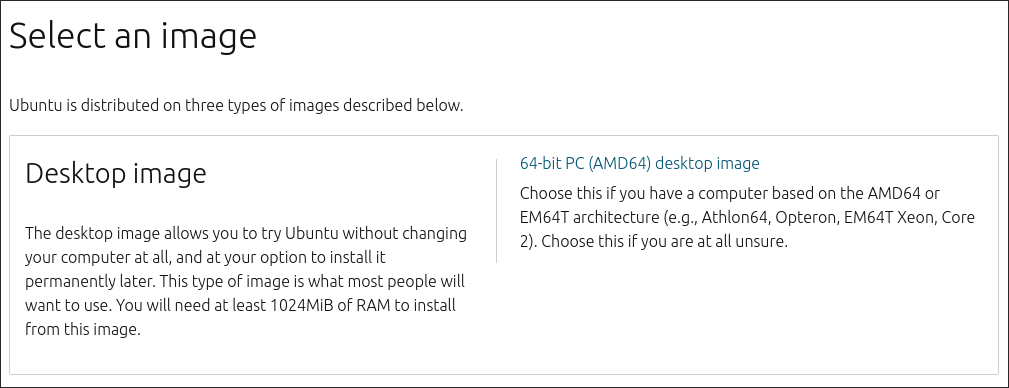
\includegraphics[width=0.7\textwidth]{images/persiapan/1.png}
    \caption{Situs resmi Ubuntu}
\end{figure}

\subsubsection{Langkah Kedua}

{\leftskip=2cm
    \hspace{1cm}Langkah kedua. Bisa kalian sesuaikan dengan praktikum kalian sendiri, jika butuh gambar, bisa salin yang di-atas (lihat raw file untuk kodenya)
    \par}

\begin{figure}[H]
    \centering
    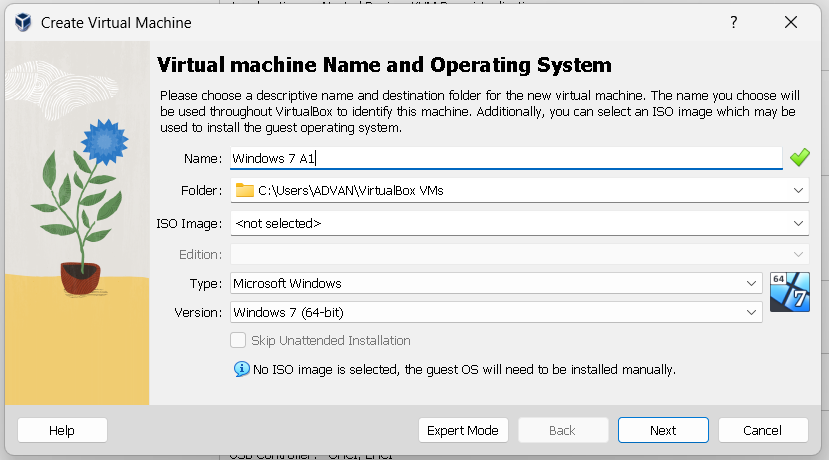
\includegraphics[width=0.7\textwidth]{images/konfigurasi-virtual-machine.png}
    \caption{Konfigurasi Virtual Machine pada Virtual Box}
\end{figure}

\subsubsection{Langkah Seterusnya}

{\leftskip=2cm
    \hspace{1cm}Langkah kedua. Bisa kalian sesuaikan dengan praktikum kalian sendiri, jika butuh gambar, bisa salin yang di-atas (lihat raw file untuk kodenya)
    \par}

\begin{figure}[H]
    \centering
    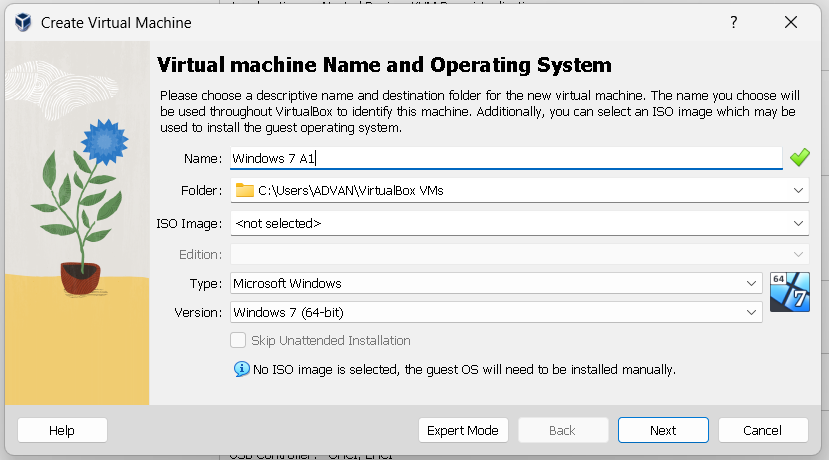
\includegraphics[width=0.7\textwidth]{images/konfigurasi-virtual-machine.png}
    \caption{Konfigurasi Virtual Machine pada Virtual Box}
\end{figure}

% ==================================================
% D. KESIMPULAN
% ==================================================

\section{Kesimpulan}

{\leftskip=0.75cm
    \hspace{1cm}Pada praktikum ini telah dilakukan ... hingga tahap ... (tulis sendiri sesuai kebutuhan). Dengan demikian, tujuan praktikum telah tercapai seluruhnya.
\par}

% ==================================================
% DAFTAR PUSTAKA
% ==================================================
\newpage
\section{Daftar Pustaka}

\printbibliography[heading=none]

% ==================================================
% SELESAI
% ==================================================

\end{document}